\chapter{Структуры данных}
\section{Дерево отрезков}
Дерево отрезков (segment tree) - структура данных, позволяющая за $O(\log{n})$ времени и $O(n)$ памяти выполнять следующие операции: \newline
\begin{itemize}
\item{Подсчётфункции для отрезка $l\dots r$}
\item{Изменение одного элемента}
\item{Изменение элементов на отрезке $l\dots r$}
\end{itemize}
\subsection*{Структура дерева отрезков}
Для данного отрезка $a = [0\dots n - 1]$ начнём делить его пополам: мы получим 2 подотрезка: $a_1 = [0\cdots \frac{|a|}{2}]$ и $a_2 = [\frac{|a|}{2} + 1\cdots n - 1]$. Посчитаем сумму на них, разобьём каждый ещё на две части и проделаем всё тоже самое для полученных подотрезков. Будем делать так, пока не получим отрезки длины 1. \newline \newline
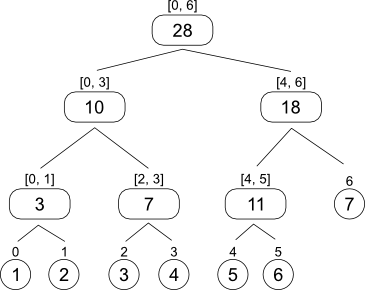
\includegraphics[height=210pt, width=400pt]{img/segment_tree} \newpage
\subsection*{Реализация дерева отрезков}
\lstinputlisting[language=C++]{src/segment_tree.cxx}